\documentclass{beamer}
\usefonttheme[onlymath]{serif}
\usepackage{amsmath}
\usepackage{amsfonts}
\usepackage[export]{adjustbox}
\usepackage[utf8]{inputenc}

% definitions
\def\H{\mathcal{H}}
\def\X{\mathbf{X}}
\def\w{\mathbf{w}}
\def\W{\mathbf{W}}
\def\const{\mathrm{const}}
\def\Var{\mathrm{Var}}
\def\tr{\mathrm{tr}}
\def\T{\top}
\def\U{\mathbf{U}}
\def\S{\mathbf{S}}
\def\V{\mathbf{V}}
\newcommand{\argmin}{\mathop{\mathrm{argmin}}}
\newcommand{\argmax}{\mathop{\mathrm{argmax}}}
\newcommand{\minimize}{\mathop{\mathrm{minimize}}}
\newcommand{\maximize}{\mathop{\mathrm{maximize}}}
\newcommand{\st}{\mathop{\mathrm{subject\,\,to}}}

%Information to be included in the title page:
\usecolortheme{seahorse}
\title{Miscellaneous Things}
\author{Thomas Bayes}
\institute{
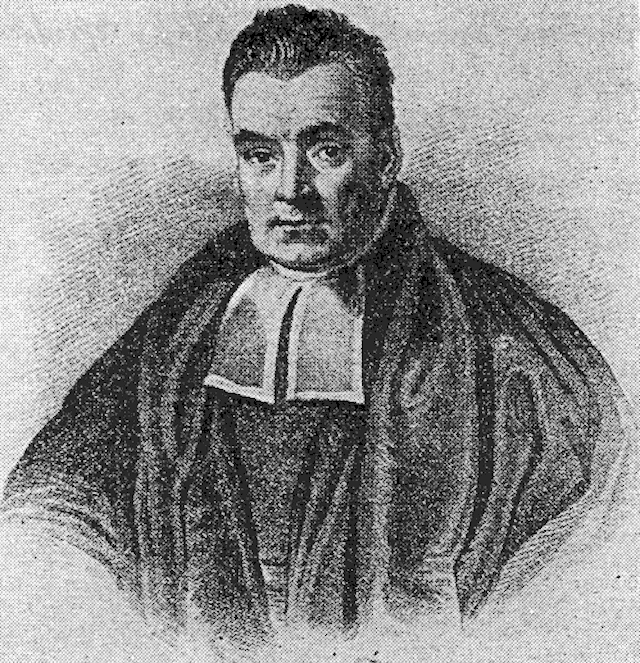
\includegraphics[height=.3\textheight]{../bayes.png}%
}
\date{\today}

    
    
\begin{document}
    
\frame{\titlepage}

\begin{frame}[allowframebreaks]{How strong is a prior?}
Suppose we want to calculate the average height $\bar{X}$ of people in the school. There can be two scenarios: 
\begin{itemize}
\item I We have no prior information about this quantity, we just go on street, observe the height of 100 people and have the estimation $\sum_{i=1}^{100}{X_i} / 100$
\item We can hire an expert on estimation of people's height and he gives us a prior distribution $\mathcal{N}(\hat{\mu}, 0.1)$.
\end{itemize}
For both scenarios, we might be inconfident about the estimation, so we still want to get more accurate results. So we still go ahead on street and observe another 100 people's height. For the reason we are going to introduce, if our experts' estimation of $\hat{\mu}$ is right, these two scenarios will lead to the same conclusion about the distribution of the average height $\mu$.

\framebreak

Because $\sigma_\text{posterior} = 1/ \sqrt{n}$, we can see that $n = 100$ for prior
distribution $\mathcal{N}(\hat{\mu},0.1)$.
\end{frame}
 
\begin{frame}{Bayes Decision Rule}
Derivation of Bayes' theorem(it is quite a shame for myself that I think it was an axiom unconsciously)
$$P(A|B) P(B) = P(B|A)P(A) \Rightarrow  P(A | B) = \frac{P(B|A) p(A)}{p(B)}$$
Bayes Decision Rule is optimal for classification mistake error:
\begin{align*}
p(\text{mistake}) & = p(x \in \mathcal{R}_1, C_2) + p(x \in \mathcal{R}_2, C_1) \\
& = \int_{\mathcal{R}_1} p(x, C_2) dx + \int_{\mathcal{R}_2} p(x, C_1)dx \\
& = \int_{\mathcal{R}_1} p(x) p(C_2|x) dx + \int_{\mathcal{R}_2} p(x) p(C_1 | x)dx
\end{align*}
Note that $p(x)$ is shared for classfication to $C_1$ or $C_2$, so we just assign the $x$ to the label whose $P(C_i | x)$ is lower.(Otherwise we can interchange the label to get lower classification error.) In more sophisticated scenarios we may not want to optimize classfication error but rather some weighted function.
\end{frame}

\begin{frame}[allowframebreaks]{Variational Inference}
We are interested in posterior distribution, but it is often too complicated and intractable, we find the member $q^\ast(\theta)$ of family $\mathcal{Q}$ over latent variables that is closest to true posterior. This transform the problem of finding the posterior to the problem of optimization.
$$q^\ast(\theta) = \argmin_{q(\theta) \in \mathcal{Q}} KL(q(\theta) || p(\theta | x))$$
Why KL divergence then?
\end{frame}

\begin{frame}[allowframebreaks]{Variational Autoencoder}

\end{frame}


\end{document}